% Options for packages loaded elsewhere
\PassOptionsToPackage{unicode}{hyperref}
\PassOptionsToPackage{hyphens}{url}
%
\documentclass[
]{book}
\usepackage{amsmath,amssymb}
\usepackage{iftex}
\ifPDFTeX
  \usepackage[T1]{fontenc}
  \usepackage[utf8]{inputenc}
  \usepackage{textcomp} % provide euro and other symbols
\else % if luatex or xetex
  \usepackage{unicode-math} % this also loads fontspec
  \defaultfontfeatures{Scale=MatchLowercase}
  \defaultfontfeatures[\rmfamily]{Ligatures=TeX,Scale=1}
\fi
\usepackage{lmodern}
\ifPDFTeX\else
  % xetex/luatex font selection
\fi
% Use upquote if available, for straight quotes in verbatim environments
\IfFileExists{upquote.sty}{\usepackage{upquote}}{}
\IfFileExists{microtype.sty}{% use microtype if available
  \usepackage[]{microtype}
  \UseMicrotypeSet[protrusion]{basicmath} % disable protrusion for tt fonts
}{}
\makeatletter
\@ifundefined{KOMAClassName}{% if non-KOMA class
  \IfFileExists{parskip.sty}{%
    \usepackage{parskip}
  }{% else
    \setlength{\parindent}{0pt}
    \setlength{\parskip}{6pt plus 2pt minus 1pt}}
}{% if KOMA class
  \KOMAoptions{parskip=half}}
\makeatother
\usepackage{xcolor}
\usepackage{color}
\usepackage{fancyvrb}
\newcommand{\VerbBar}{|}
\newcommand{\VERB}{\Verb[commandchars=\\\{\}]}
\DefineVerbatimEnvironment{Highlighting}{Verbatim}{commandchars=\\\{\}}
% Add ',fontsize=\small' for more characters per line
\usepackage{framed}
\definecolor{shadecolor}{RGB}{248,248,248}
\newenvironment{Shaded}{\begin{snugshade}}{\end{snugshade}}
\newcommand{\AlertTok}[1]{\textcolor[rgb]{0.94,0.16,0.16}{#1}}
\newcommand{\AnnotationTok}[1]{\textcolor[rgb]{0.56,0.35,0.01}{\textbf{\textit{#1}}}}
\newcommand{\AttributeTok}[1]{\textcolor[rgb]{0.13,0.29,0.53}{#1}}
\newcommand{\BaseNTok}[1]{\textcolor[rgb]{0.00,0.00,0.81}{#1}}
\newcommand{\BuiltInTok}[1]{#1}
\newcommand{\CharTok}[1]{\textcolor[rgb]{0.31,0.60,0.02}{#1}}
\newcommand{\CommentTok}[1]{\textcolor[rgb]{0.56,0.35,0.01}{\textit{#1}}}
\newcommand{\CommentVarTok}[1]{\textcolor[rgb]{0.56,0.35,0.01}{\textbf{\textit{#1}}}}
\newcommand{\ConstantTok}[1]{\textcolor[rgb]{0.56,0.35,0.01}{#1}}
\newcommand{\ControlFlowTok}[1]{\textcolor[rgb]{0.13,0.29,0.53}{\textbf{#1}}}
\newcommand{\DataTypeTok}[1]{\textcolor[rgb]{0.13,0.29,0.53}{#1}}
\newcommand{\DecValTok}[1]{\textcolor[rgb]{0.00,0.00,0.81}{#1}}
\newcommand{\DocumentationTok}[1]{\textcolor[rgb]{0.56,0.35,0.01}{\textbf{\textit{#1}}}}
\newcommand{\ErrorTok}[1]{\textcolor[rgb]{0.64,0.00,0.00}{\textbf{#1}}}
\newcommand{\ExtensionTok}[1]{#1}
\newcommand{\FloatTok}[1]{\textcolor[rgb]{0.00,0.00,0.81}{#1}}
\newcommand{\FunctionTok}[1]{\textcolor[rgb]{0.13,0.29,0.53}{\textbf{#1}}}
\newcommand{\ImportTok}[1]{#1}
\newcommand{\InformationTok}[1]{\textcolor[rgb]{0.56,0.35,0.01}{\textbf{\textit{#1}}}}
\newcommand{\KeywordTok}[1]{\textcolor[rgb]{0.13,0.29,0.53}{\textbf{#1}}}
\newcommand{\NormalTok}[1]{#1}
\newcommand{\OperatorTok}[1]{\textcolor[rgb]{0.81,0.36,0.00}{\textbf{#1}}}
\newcommand{\OtherTok}[1]{\textcolor[rgb]{0.56,0.35,0.01}{#1}}
\newcommand{\PreprocessorTok}[1]{\textcolor[rgb]{0.56,0.35,0.01}{\textit{#1}}}
\newcommand{\RegionMarkerTok}[1]{#1}
\newcommand{\SpecialCharTok}[1]{\textcolor[rgb]{0.81,0.36,0.00}{\textbf{#1}}}
\newcommand{\SpecialStringTok}[1]{\textcolor[rgb]{0.31,0.60,0.02}{#1}}
\newcommand{\StringTok}[1]{\textcolor[rgb]{0.31,0.60,0.02}{#1}}
\newcommand{\VariableTok}[1]{\textcolor[rgb]{0.00,0.00,0.00}{#1}}
\newcommand{\VerbatimStringTok}[1]{\textcolor[rgb]{0.31,0.60,0.02}{#1}}
\newcommand{\WarningTok}[1]{\textcolor[rgb]{0.56,0.35,0.01}{\textbf{\textit{#1}}}}
\usepackage{longtable,booktabs,array}
\usepackage{calc} % for calculating minipage widths
% Correct order of tables after \paragraph or \subparagraph
\usepackage{etoolbox}
\makeatletter
\patchcmd\longtable{\par}{\if@noskipsec\mbox{}\fi\par}{}{}
\makeatother
% Allow footnotes in longtable head/foot
\IfFileExists{footnotehyper.sty}{\usepackage{footnotehyper}}{\usepackage{footnote}}
\makesavenoteenv{longtable}
\usepackage{graphicx}
\makeatletter
\def\maxwidth{\ifdim\Gin@nat@width>\linewidth\linewidth\else\Gin@nat@width\fi}
\def\maxheight{\ifdim\Gin@nat@height>\textheight\textheight\else\Gin@nat@height\fi}
\makeatother
% Scale images if necessary, so that they will not overflow the page
% margins by default, and it is still possible to overwrite the defaults
% using explicit options in \includegraphics[width, height, ...]{}
\setkeys{Gin}{width=\maxwidth,height=\maxheight,keepaspectratio}
% Set default figure placement to htbp
\makeatletter
\def\fps@figure{htbp}
\makeatother
\setlength{\emergencystretch}{3em} % prevent overfull lines
\providecommand{\tightlist}{%
  \setlength{\itemsep}{0pt}\setlength{\parskip}{0pt}}
\setcounter{secnumdepth}{5}
\usepackage{booktabs}
\usepackage{amsthm}
\makeatletter
\def\thm@space@setup{%
  \thm@preskip=8pt plus 2pt minus 4pt
  \thm@postskip=\thm@preskip
}
\makeatother
\ifLuaTeX
  \usepackage{selnolig}  % disable illegal ligatures
\fi
\usepackage[]{natbib}
\bibliographystyle{apalike}
\usepackage{bookmark}
\IfFileExists{xurl.sty}{\usepackage{xurl}}{} % add URL line breaks if available
\urlstyle{same}
\hypersetup{
  pdftitle={Face lab book},
  pdfauthor={Face lab},
  hidelinks,
  pdfcreator={LaTeX via pandoc}}

\title{Face lab book}
\author{Face lab}
\date{2024-11-07}

\begin{document}
\maketitle

{
\setcounter{tocdepth}{1}
\tableofcontents
}
\chapter{简介}\label{ux7b80ux4ecb}

这是面孔实验室的实验手册,目前主要尝试介绍一些常用的软件或技术。

实验室目前常用的软件有:\\
- Chapter \ref{jamovi}: Jamovi\\
- Chapter \ref{zotero}: Zotero

\chapter{Jamovi}\label{jamovi}

汇总:沈佳欣、张宇杰\\
更新于:2024 Nov 07

\section{方差分析}\label{ux65b9ux5deeux5206ux6790}

导入数据后,依次点击``分析''\,``方差分析''选项,然后在弹出的选项栏中选择适当的方差分析方法。前五个为参数检验方法,后两个为非参数检验方法,它们分别对应统计课本中的克-瓦氏单向方差分析和弗里德曼两因素等级方差分析。

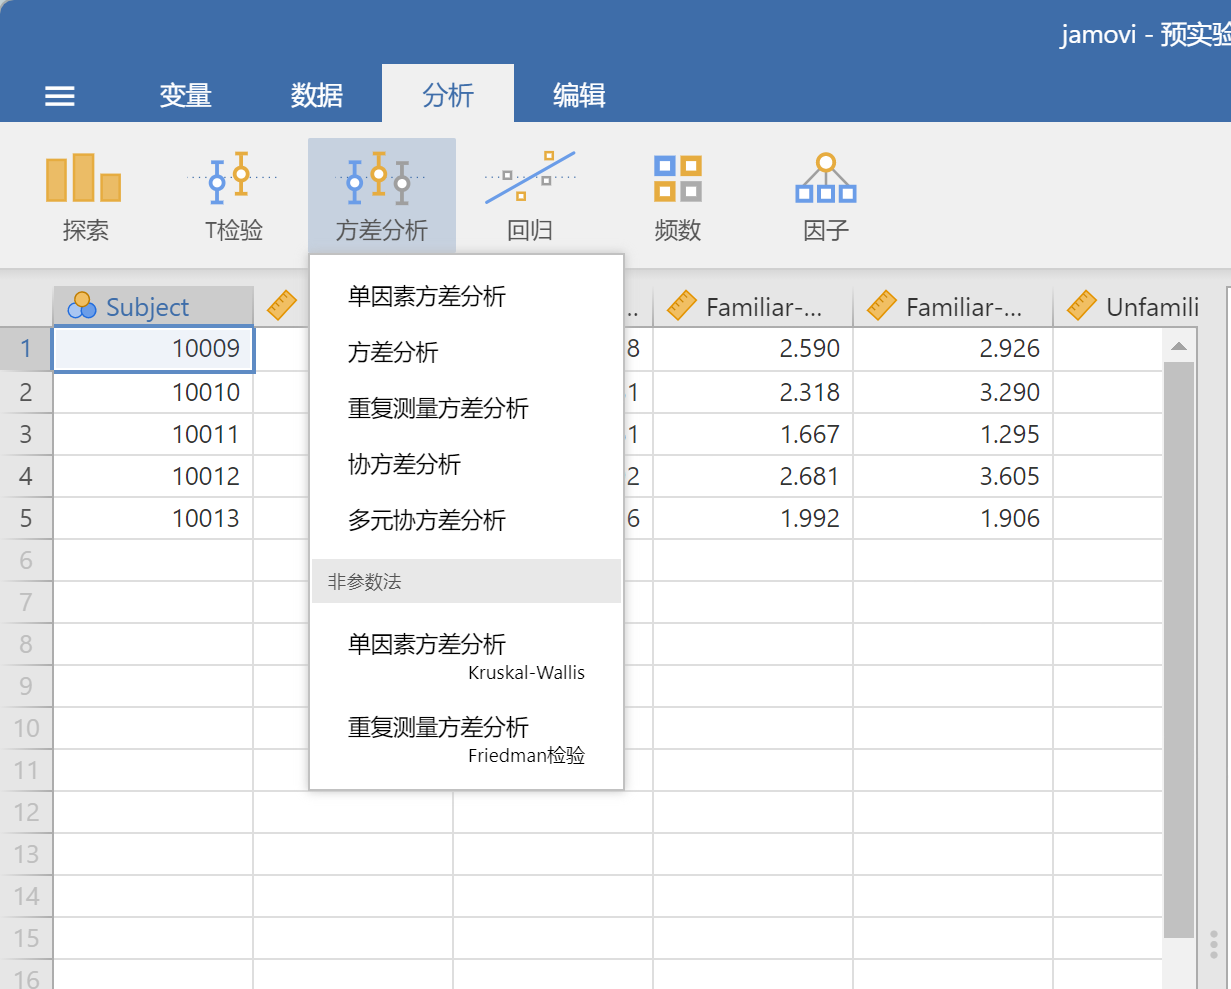
\includegraphics{img/jamovi/anova.png}

此次以重复测量方差分析为例。在下图左侧的界面里,左侧是我们数据的名称,右侧的``重复测量因子''是指在研究中设置的``被试内自变量''。在本例中,我们有三个``被试内自变量'',每个自变量都有两个水平。例如我们将``重复测量因子1''定义为Familiar,它包括``familiar''和``unfamiliar''两个水平。

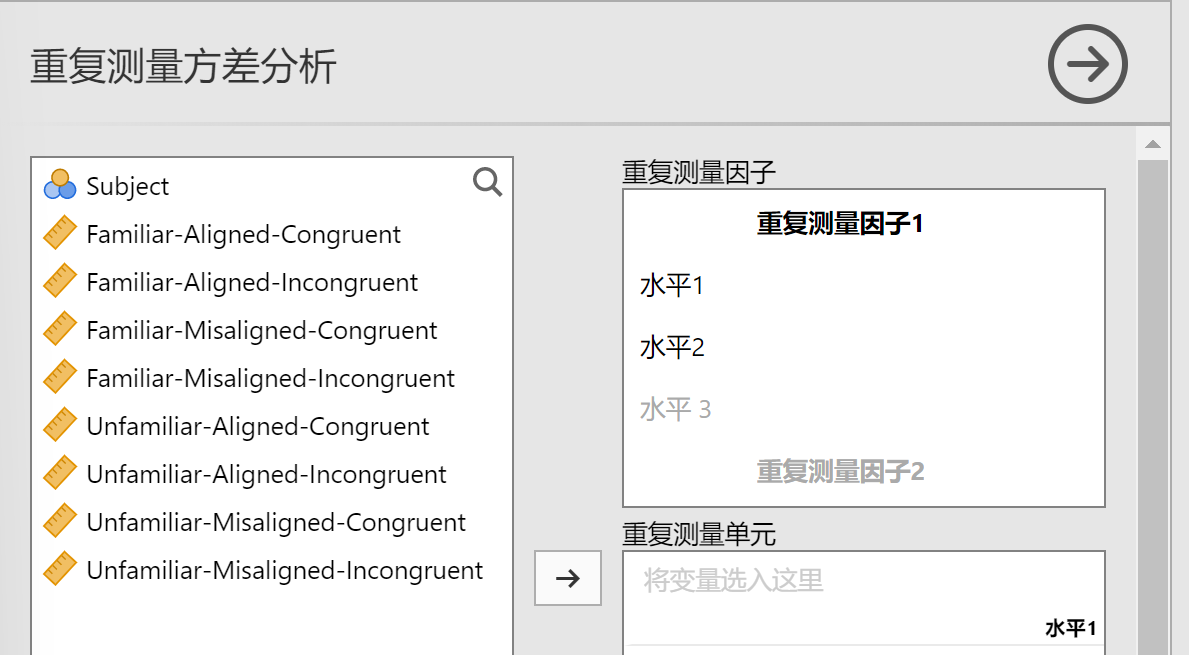
\includegraphics{img/jamovi/rmanova-factor.png}\\
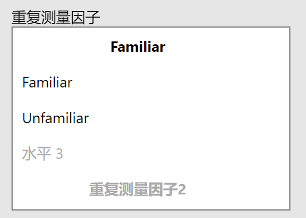
\includegraphics{img/jamovi/rmanova-factorlevels.png}

定义好重复测量因子后,``重复测量单元''中会出现各个自变量水平的组合,而``重复测量单元''也就是指研究中的各种实验条件。在本例中我们的实验是一个2 * 2 * 2的被试内设计,所以共有8种实验条件,我们需要做的是将数据拖入其对应的重复测量单元中。

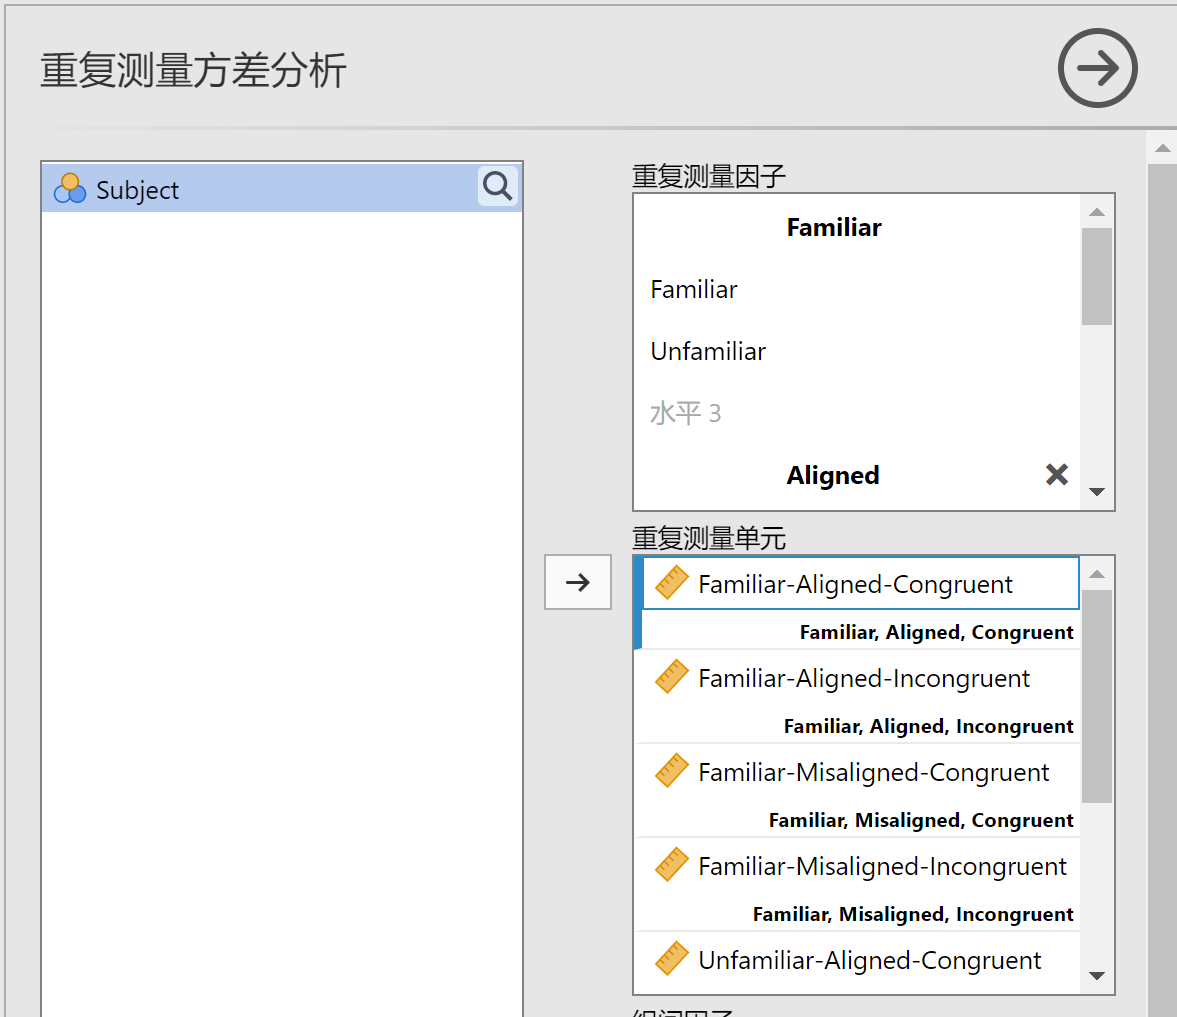
\includegraphics{img/jamovi/rmanova-factorlevels2.png}

接下来我们要选择效应量为``偏η²值'',以及确定因变量标签。本例中因变量标签为``d-prime''.

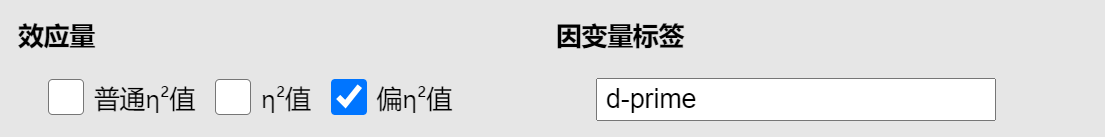
\includegraphics{img/jamovi/rmanova-dv.png}

下面的五个选项里,我们应当关注的主要是``适用条件判断''和``事后检验''。

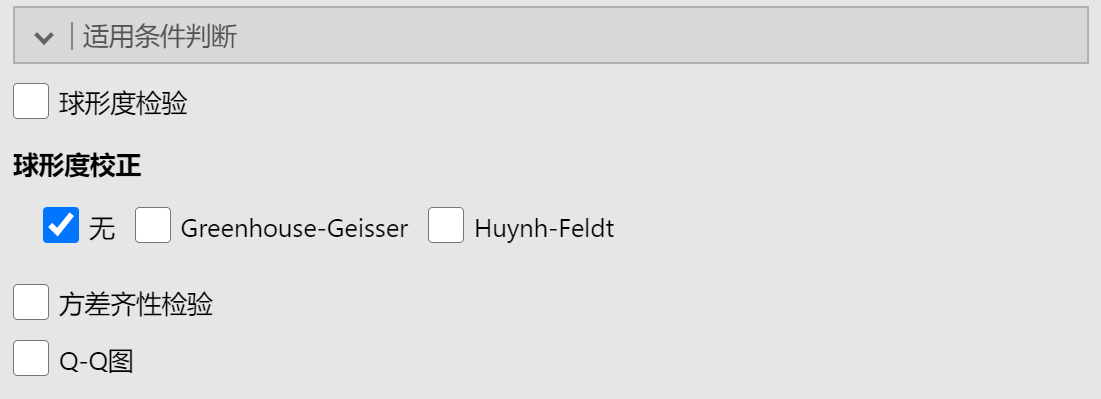
\includegraphics{img/jamovi/rmanova-sphericity.png}

对本专业来说,在这一栏中较为重要的是``方差齐性检验'',如果变量中涉及被试间变量,那么应当进行方差齐性检验。但由于本例中的变量都是被试内变量,所以无需进行方差齐性检验。其他几个选项可以根据研究所需进行选取。

所有设定完成后,jamovi会在右侧呈现数据分析结果。

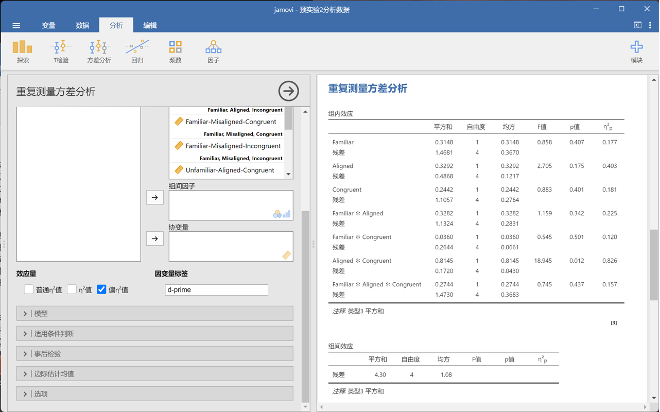
\includegraphics{img/jamovi/rmanova-result.png}

\section{简单效应分析}\label{ux7b80ux5355ux6548ux5e94ux5206ux6790}

这一部分承接上述重复测量方差分析。在本例中,当我们在jamovi中确定好了``重复测量因子''即``被试内变量''和``重复测量单元''即``实验条件''后,我们可以看到右侧的结果栏中就可以呈现统计结果,如果某两个或几个变量之间存在显著的交互作用,那么我们应当进行事后检验,以确定一个变量在与它有交互作用的另一个变量的哪些水平上显著,哪些水平上不显著。我们需要选择下列五个选项中的``事后检验''。

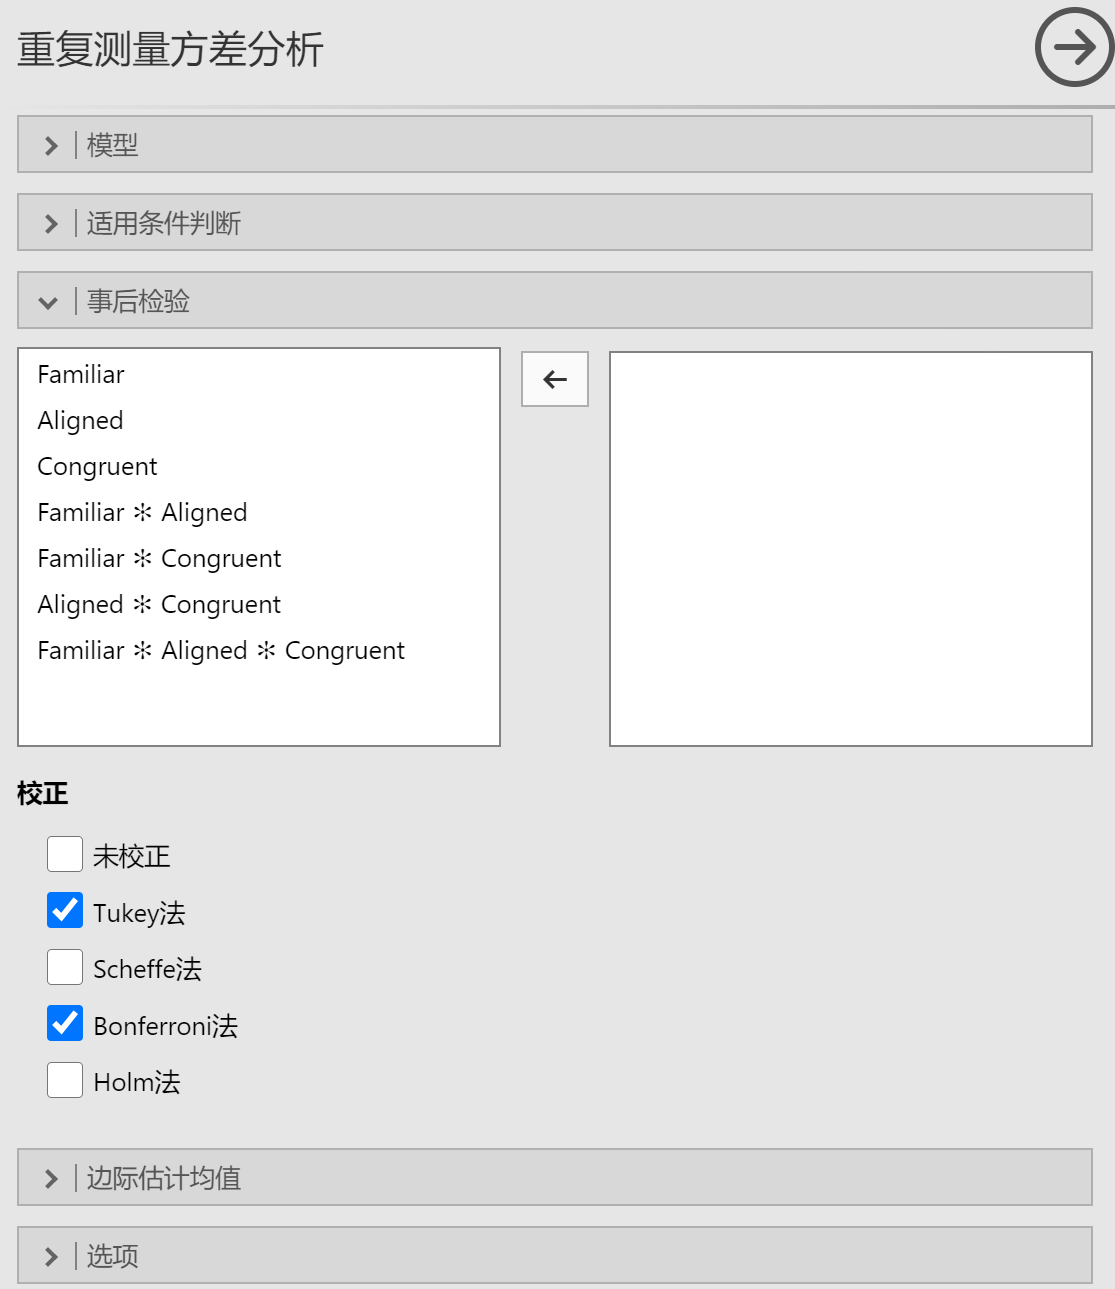
\includegraphics{img/jamovi/rmanova-posthoc.png}

选择需要进行事后检验的交互变量,并按照需要选择恰当的校正方法。

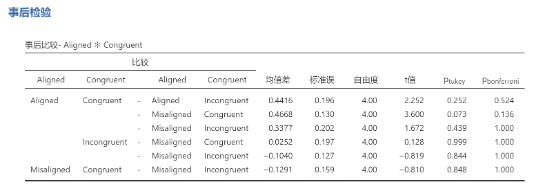
\includegraphics{img/jamovi/rmanova-posthoc-results.png}

右侧生成的结果的最右边两列就是jamovi按照我们选择的Tukey法和Bonferron法计算出的统计值。

\section{t检验}\label{tux68c0ux9a8c}

\begin{itemize}
\tightlist
\item
  首先,导入数据
\item
  其次,点击选项栏的分析,选择对应的t检验
\end{itemize}

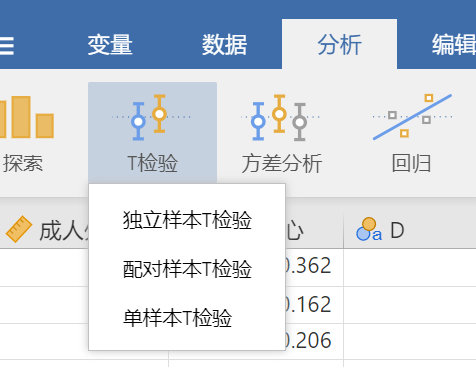
\includegraphics{img/jamovi/ttest.png}

\begin{itemize}
\tightlist
\item
  接着,选择要分析的变量
\end{itemize}

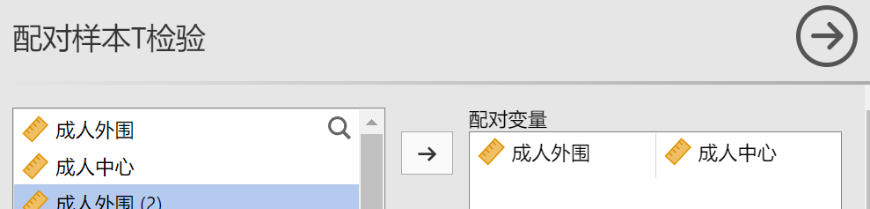
\includegraphics{img/jamovi/ttest-compare.png}

\begin{itemize}
\tightlist
\item
  然后,可以按需勾选,描述就是分析数据的均值、标准差、标准误等描述性数据;描述图就是生成图表
\end{itemize}

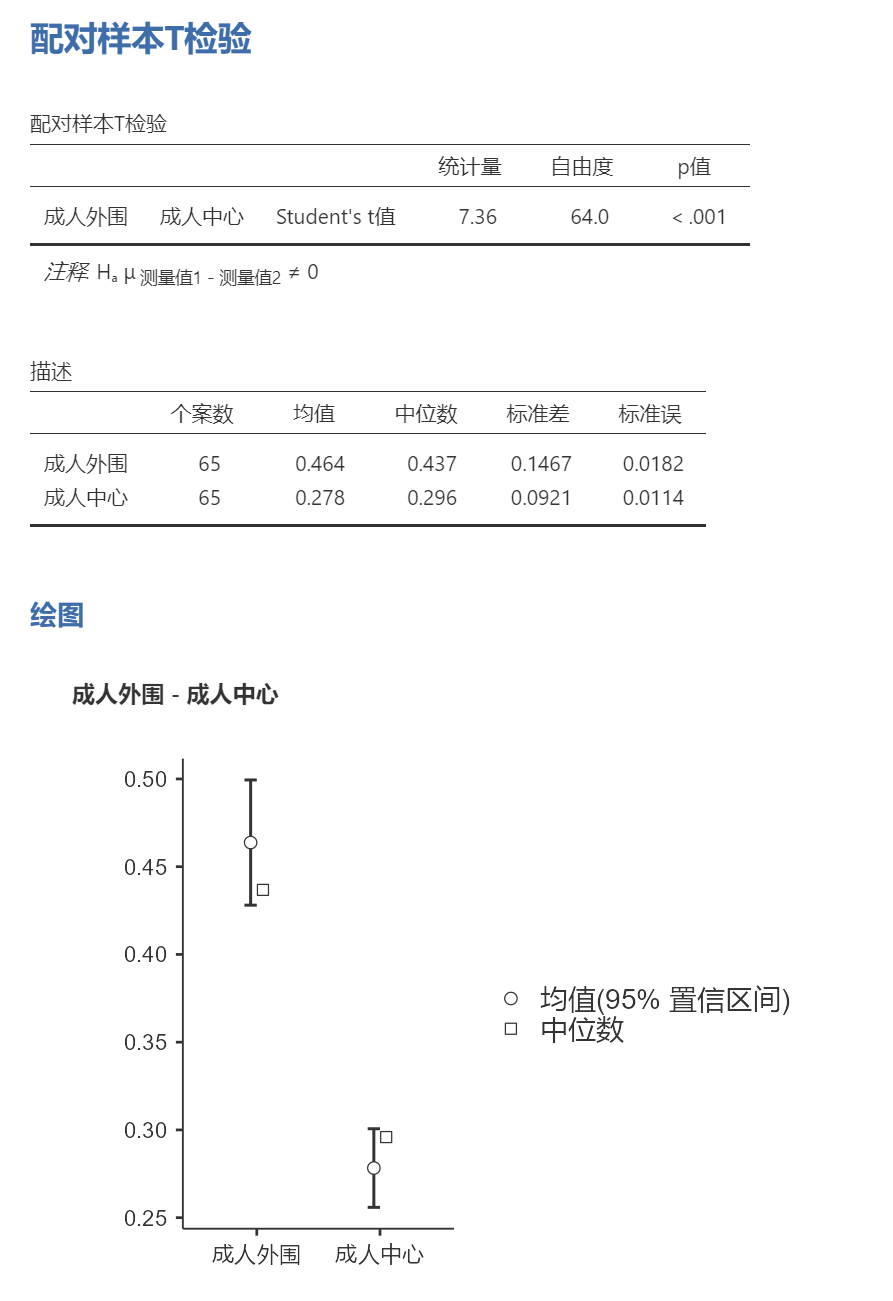
\includegraphics{img/jamovi/ttest-results.png}

\section{额外模块推荐}\label{ux989dux5916ux6a21ux5757ux63a8ux8350}

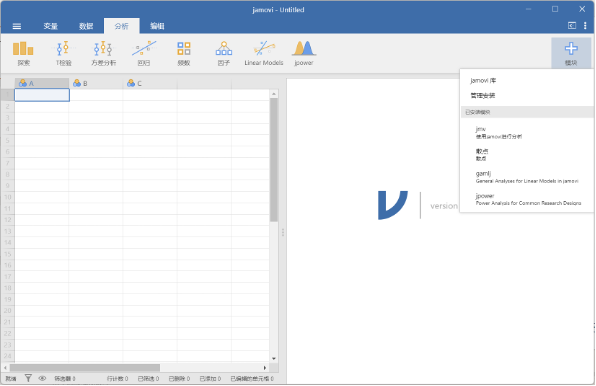
\includegraphics{img/jamovi/modules.png}\\
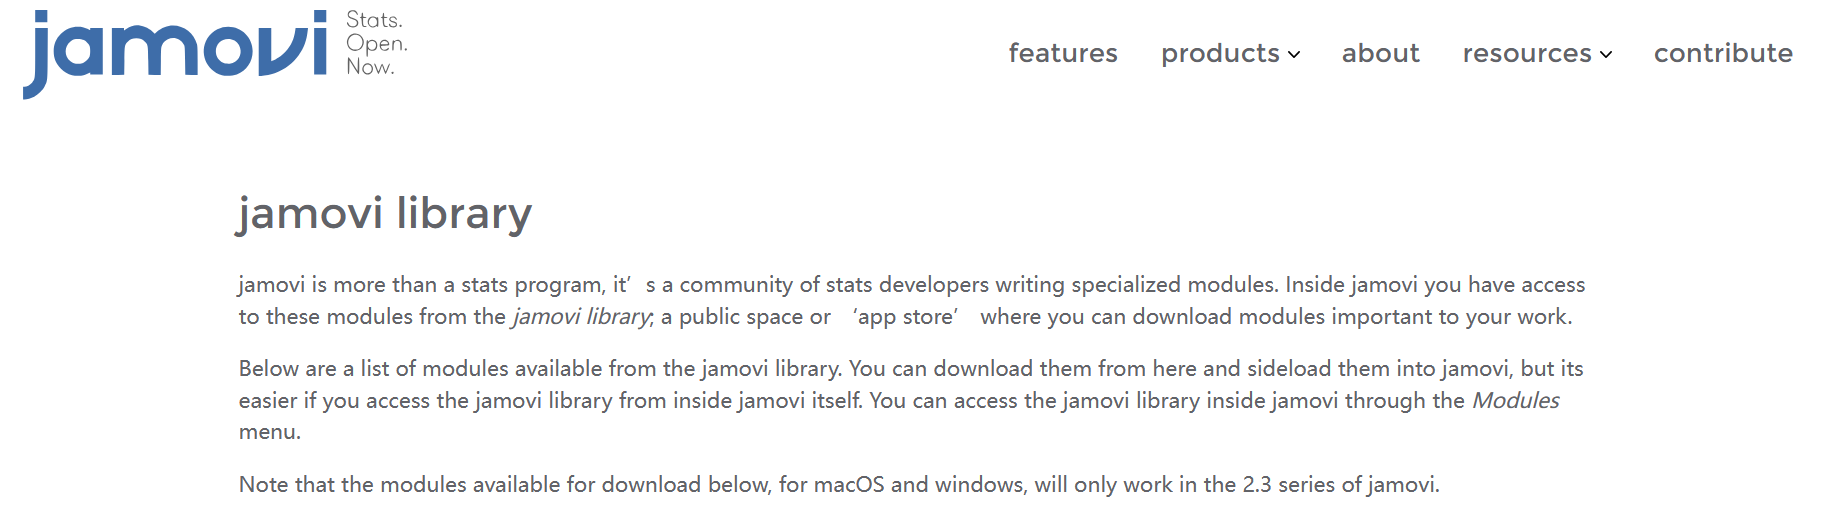
\includegraphics{img/jamovi/modules-library.png}

可以通过jamovi官网下载自己所需要的库。这是网址:\url{https://www.jamovi.org/library.html}

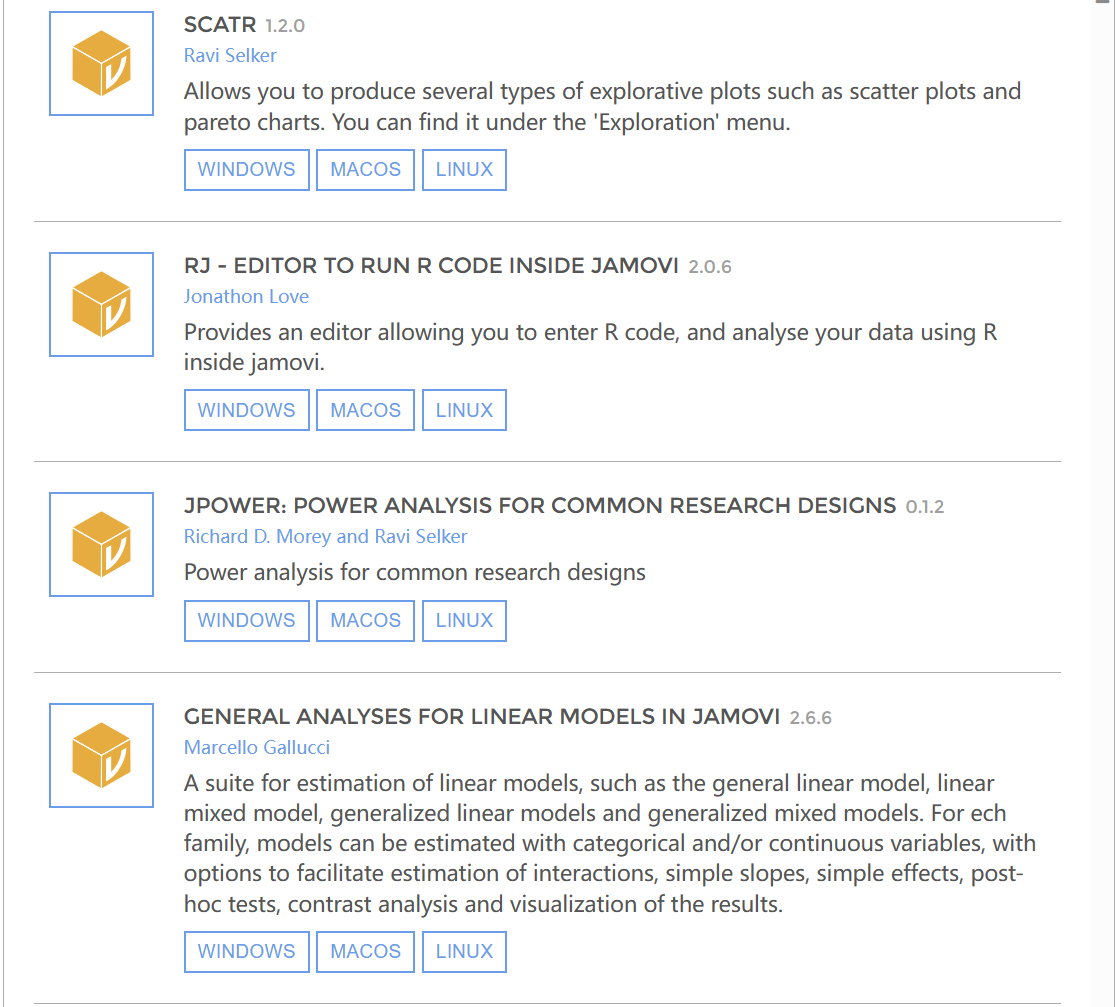
\includegraphics{img/jamovi/modules1.png}\\
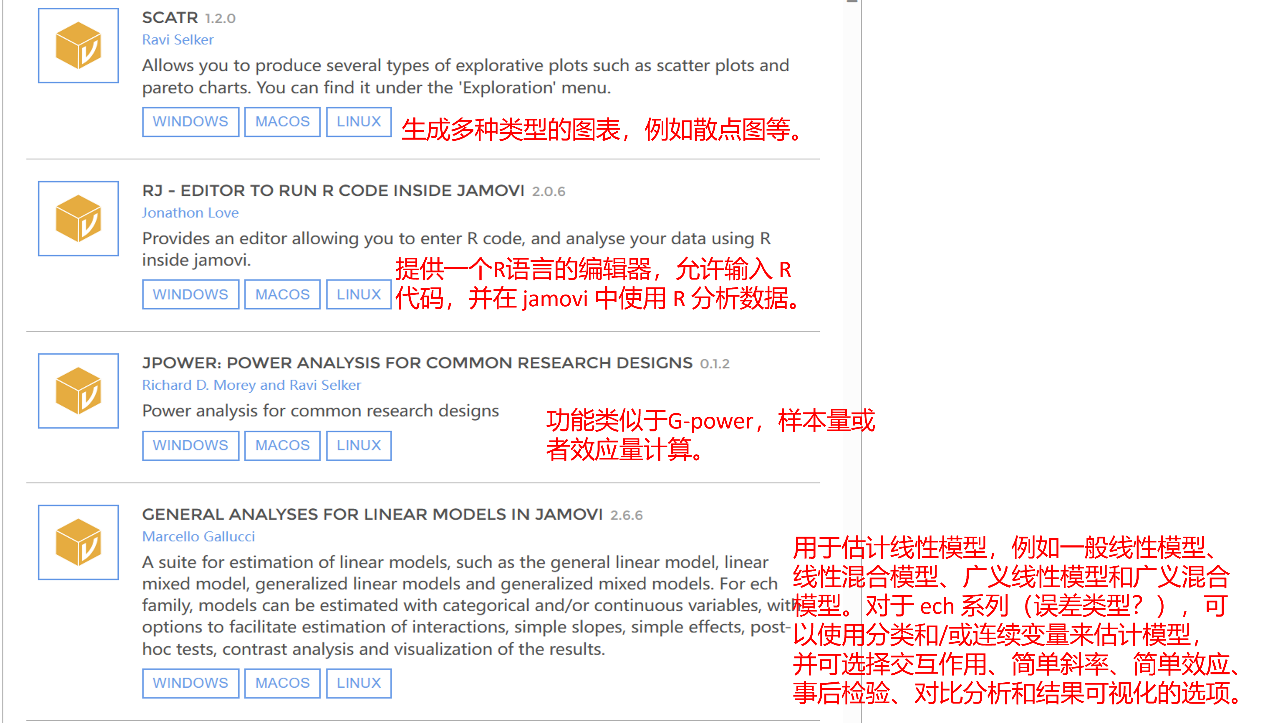
\includegraphics{img/jamovi/modules2.png}\\
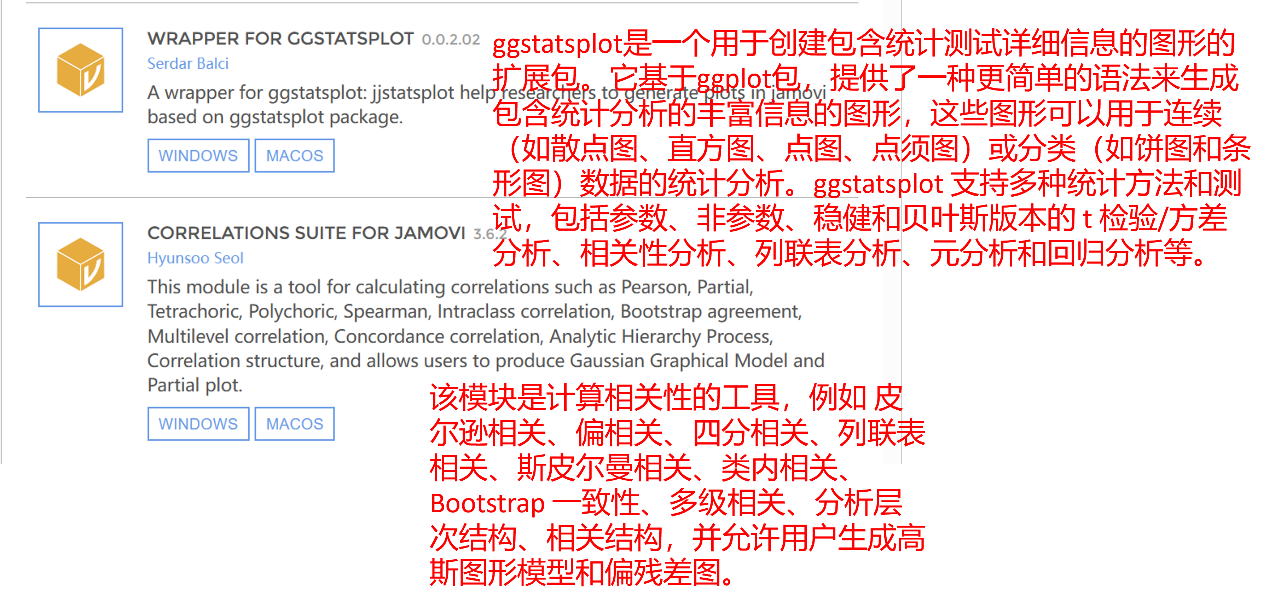
\includegraphics{img/jamovi/modules3.png}\\
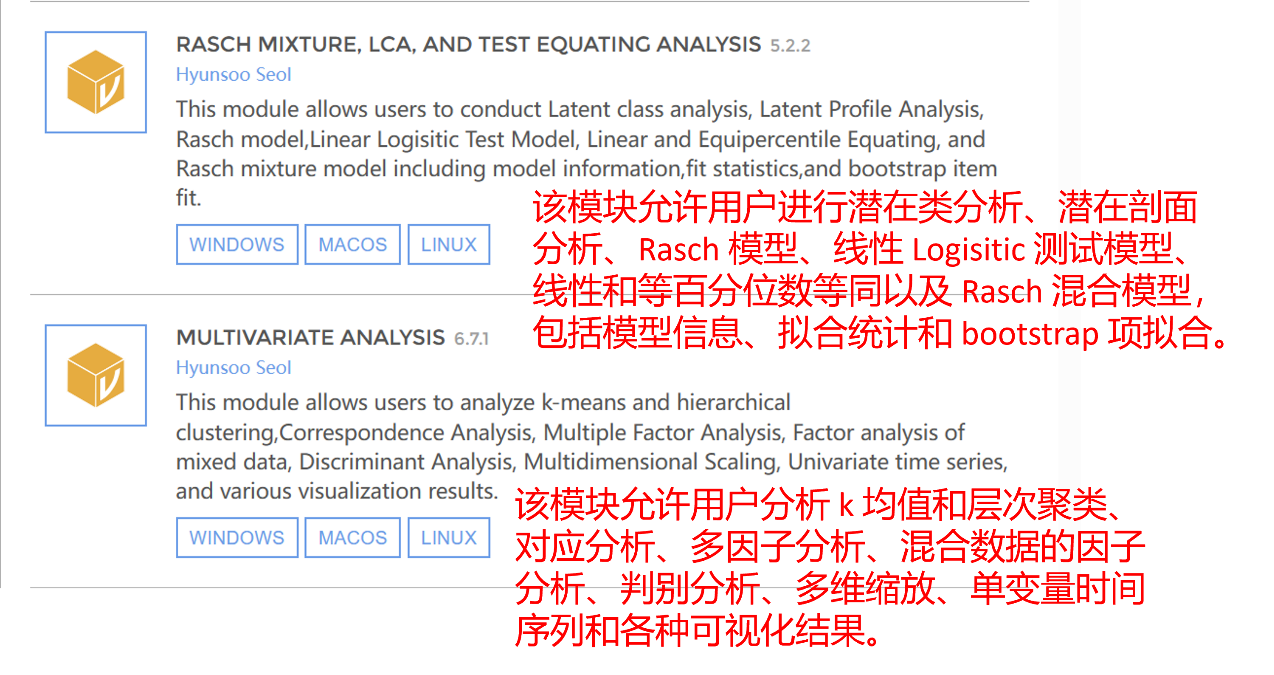
\includegraphics{img/jamovi/modules4.png}

\chapter{Zotero}\label{zotero}

汇总:郭沫然\\
更新于:2024 Nov 07

\chapter*{Archive}\label{archive}
\addcontentsline{toc}{chapter}{Archive}

You can label chapter and section titles using \texttt{\{\#label\}} after them, e.g., we can reference Chapter \ref{intro}. If you do not manually label them, there will be automatic labels anyway, e.g., Chapter \ref{methods}.

Figures and tables with captions will be placed in \texttt{figure} and \texttt{table} environments, respectively.

\begin{Shaded}
\begin{Highlighting}[]
\FunctionTok{par}\NormalTok{(}\AttributeTok{mar =} \FunctionTok{c}\NormalTok{(}\DecValTok{4}\NormalTok{, }\DecValTok{4}\NormalTok{, .}\DecValTok{1}\NormalTok{, .}\DecValTok{1}\NormalTok{))}
\FunctionTok{plot}\NormalTok{(pressure, }\AttributeTok{type =} \StringTok{\textquotesingle{}b\textquotesingle{}}\NormalTok{, }\AttributeTok{pch =} \DecValTok{19}\NormalTok{)}
\end{Highlighting}
\end{Shaded}

\begin{figure}

{\centering 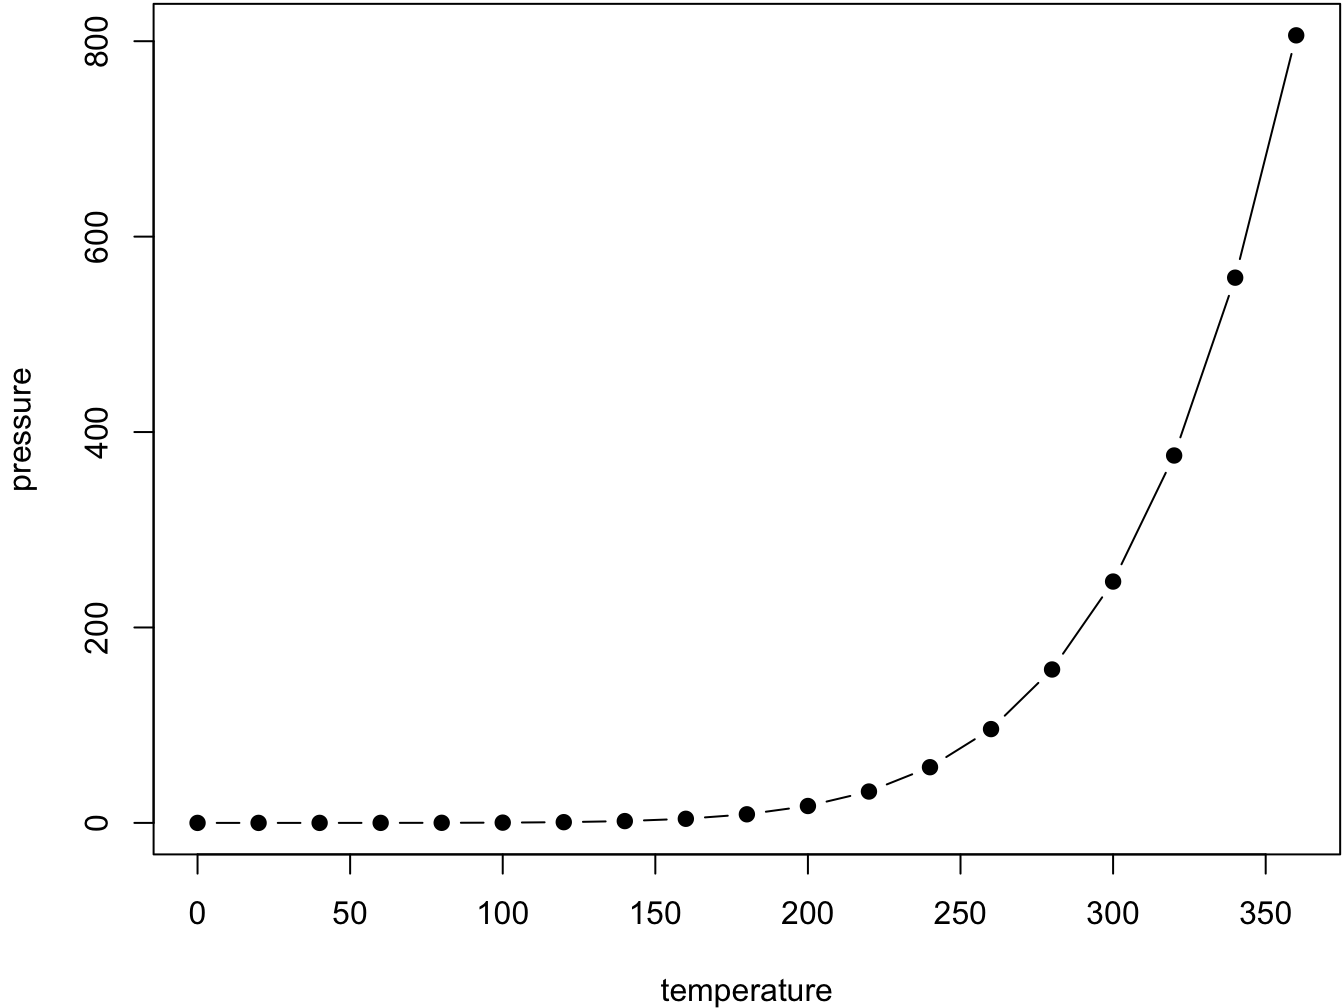
\includegraphics[width=0.8\linewidth]{face_lab_book_files/figure-latex/nice-fig-1} 

}

\caption{Here is a nice figure!}\label{fig:nice-fig}
\end{figure}

Reference a figure by its code chunk label with the \texttt{fig:} prefix, e.g., see Figure \ref{fig:nice-fig}. Similarly, you can reference tables generated from \texttt{knitr::kable()}, e.g., see Table \ref{tab:nice-tab}.

\begin{Shaded}
\begin{Highlighting}[]
\NormalTok{knitr}\SpecialCharTok{::}\FunctionTok{kable}\NormalTok{(}
  \FunctionTok{head}\NormalTok{(iris, }\DecValTok{20}\NormalTok{), }\AttributeTok{caption =} \StringTok{\textquotesingle{}Here is a nice table!\textquotesingle{}}\NormalTok{,}
  \AttributeTok{booktabs =} \ConstantTok{TRUE}
\NormalTok{)}
\end{Highlighting}
\end{Shaded}

\begin{table}

\caption{\label{tab:nice-tab}Here is a nice table!}
\centering
\begin{tabular}[t]{rrrrl}
\toprule
Sepal.Length & Sepal.Width & Petal.Length & Petal.Width & Species\\
\midrule
5.1 & 3.5 & 1.4 & 0.2 & setosa\\
4.9 & 3.0 & 1.4 & 0.2 & setosa\\
4.7 & 3.2 & 1.3 & 0.2 & setosa\\
4.6 & 3.1 & 1.5 & 0.2 & setosa\\
5.0 & 3.6 & 1.4 & 0.2 & setosa\\
\addlinespace
5.4 & 3.9 & 1.7 & 0.4 & setosa\\
4.6 & 3.4 & 1.4 & 0.3 & setosa\\
5.0 & 3.4 & 1.5 & 0.2 & setosa\\
4.4 & 2.9 & 1.4 & 0.2 & setosa\\
4.9 & 3.1 & 1.5 & 0.1 & setosa\\
\addlinespace
5.4 & 3.7 & 1.5 & 0.2 & setosa\\
4.8 & 3.4 & 1.6 & 0.2 & setosa\\
4.8 & 3.0 & 1.4 & 0.1 & setosa\\
4.3 & 3.0 & 1.1 & 0.1 & setosa\\
5.8 & 4.0 & 1.2 & 0.2 & setosa\\
\addlinespace
5.7 & 4.4 & 1.5 & 0.4 & setosa\\
5.4 & 3.9 & 1.3 & 0.4 & setosa\\
5.1 & 3.5 & 1.4 & 0.3 & setosa\\
5.7 & 3.8 & 1.7 & 0.3 & setosa\\
5.1 & 3.8 & 1.5 & 0.3 & setosa\\
\bottomrule
\end{tabular}
\end{table}

You can write citations, too. For example, we are using the \textbf{bookdown} package \citep{R-bookdown} in this sample book, which was built on top of R Markdown and \textbf{knitr} \citep{xie2015}.

  \bibliography{book.bib}

\end{document}
